\documentclass[12pt%
%,draft%
,aspectratio=169%
]{beamer}
%
\usepackage{fontspec}
\defaultfontfeatures{Ligatures=TeX}
%\setsansfont{Liberation Sans}
\usepackage{polyglossia}
\setdefaultlanguage{ngerman}
% Alternative template for talks of the Freie Universität Berlin.
% Created by Leonard R. König, <leonard.koenig@fu-berlin.de> following the
% guidelines on www.fu-berlin.de/cd
%
% (c) Leonard König, CC BY 4.0
%
% This template was written against UTF-8 capable LaTeX engines, specifically
% LuaLaTeX.

% Trying to get rather close to the ppt/odp template:
%  http://www.fu-berlin.de/sites/cd/downloads_container/PowerPoint_Praesentation_Anleitung.pdf

%%% font styles
\setbeamerfont{frametitle}{series=\bfseries}
\setbeamerfont{footline}{series=\bfseries}
\setbeamerfont{headline}{series=\bfseries}
\setbeamerfont{alerted text}{series=\bfseries}
%%%

% colordefs
\definecolor{fu_darkblue}{RGB}{0,51,102}
\definecolor{fu_seablue}{RGB}{0,102,204}
\definecolor{fu_lightblue}{RGB}{204,214,224}
\definecolor{fu_green}{RGB}{153,204,0}
\definecolor{fu_lightgrey}{RGB}{128,128,128}
\definecolor{fu_grey}{RGB}{95,95,95}
%
\definecolor{fu_red}{RGB}{204, 0, 0} % red text (used by \alert)
%%% end colordefs

%%% colors
\setbeamercolor*{title}{fg=fu_darkblue}
\setbeamercolor*{subtitle}{fg=fu_seablue}
\setbeamercolor*{frametitle}{fg=fu_darkblue}
\setbeamercolor*{footline}{fg=fu_grey,bg=fu_lightblue}
\setbeamercolor*{headline}{fg=fu_grey}

\setbeamercolor*{normal text}{fg=black}
\setbeamercolor*{alerted text}{fg=fu_red}
\setbeamercolor*{example text}{fg=fu_green}
\setbeamercolor*{structure}{fg=fu_darkblue}

\setbeamercolor*{block title}{fg=white,bg=black!50}
\setbeamercolor*{block title alerted}{fg=white,bg=black!50}
\setbeamercolor*{block title example}{fg=white,bg=black!50}

\setbeamercolor*{block body}{bg=black!10}
\setbeamercolor*{block body alerted}{bg=black!10}
\setbeamercolor*{block body example}{bg=black!10}

\setbeamercolor{bibliography entry author}{fg=fu_darkblue}

\setbeamercolor{item}{fg=fu_darkblue}
\setbeamercolor{navigation symbols}{fg=fu_lightgrey,bg=fu_grey}
%%% end colors

%%% title page
% Display logo (if exists) and right next to it, put our title + subtitle
\defbeamertemplate*{title page}{fu_titlepage}
{%
	\hskip .3\textheight
	\begin{minipage}[.4\textheight]{\textwidth}
		\begin{minipage}[.4\textheight]{0.25\textwidth}
			\inserttitlegraphic
		\end{minipage}%
		\begin{minipage}[.4\textheight]{0.75\textwidth}
			\begin{beamercolorbox}{title}
				\usebeamerfont{title}\inserttitle\par%
			\end{beamercolorbox}
			\vfill
			\ifx\insertsubtitle
				\@empty%
			\else
				\begin{beamercolorbox}{subtitle}
					\usebeamerfont{subtitle}\insertsubtitle\par
				\end{beamercolorbox}
			\fi
		\end{minipage}
	\end{minipage}%
	\hskip .3\textheight
}
%%% end title page

%%% headline
% display title, author and institute on the left;
% logo on the right.
\newcommand{\headlinetext}
{%
	\inserttitle\\[0.3em]%
	\insertauthor, %
	\insertshortinstitute
}
\newlength{\headlinewidth}
\setlength{\headlinewidth}{\paperwidth}
\addtolength{\headlinewidth}{-2\marginparsep}
\setbeamertemplate{headline}
{%
	\begin{beamercolorbox}[wd=\paperwidth]{headline}%
		\vskip5pt
		{\hspace*{\marginparsep}}%
		\parbox{.5\headlinewidth}
		{%
			\usebeamertemplate{title in head/foot}%
			\headlinetext%
		}%
		\begin{minipage}{.5\headlinewidth}%
			\hfill\usebeamertemplate*{logo}
		\end{minipage}%
		{\hspace*{\marginparsep}}%
	\end{beamercolorbox}%
}
%%% end headline

%%% footline
% title + date on the left, frame number on the right
\newcommand{\footlinetext}
{%
	\usebeamerfont{shorttitle}\insertshorttitle, %
	\usebeamerfont{shortdate}\insertshortdate
}
\setbeamertemplate{footline}
{%
	\begin{beamercolorbox}{footline}
		\vskip2pt
		\hspace{\marginparsep}%
		\footlinetext\hfill%
		\insertframenumber%
		\hspace{\marginparsep}
		\vskip2pt
	\end{beamercolorbox}%
}
%%% end footline

% don't use default templates for sidebars
\setbeamertemplate{sidebar right}{}
\setbeamertemplate{sidebar left}{}
\setbeamertemplate{title page}[fu_titlepage]
\usepackage{amsmath}
\usepackage{amsfonts}
\usepackage{amssymb}
\usepackage{graphicx}
\usepackage{algorithm}
\usepackage[noend]{algpseudocode}
%\usepackage{algorithmic}
\usepackage{tikz}
\usetikzlibrary{arrows,shapes,automata,petri,positioning,calc}
\usepackage{graphicx}
\usepackage{subfig}
\usepackage{pgfplots}
\usepackage{ stmaryrd }
\usepackage[normalem]{ulem}
\usepackage{circuitikz}
\usepackage{bohr}
\usepackage{csquotes}

\setbeamercolor{block title}{use=structure,fg=white,bg=structure.fg!75!black}
\setbeamercolor{block body}{parent=normal text,use=block title,bg=block title.bg!10!bg}


\author{Benjamin Tröster}
\title[Zahlendarstellung]{Zahlendarstellung}
%\subtitle[Markov Models]{...}
%\pgfdeclareimage{titlegraphic}{../res/dwarf_logo2.png}
%\titlegraphic{\pgfuseimage{titlegraphic}}
%\date{}
%\subject{}
%
% FU settings
\institute[HTW Berlin]{Hochschule für Technik und Wirtschaft Berlin}
%\pgfdeclareimage[height=0.9cm]{logo}{../res/dwarf_logo}
%\logo{\pgfuseimage{logo}}
%
\usepackage[
backend=biber,
citestyle=alphabetic,bibstyle=authoryear
]{biblatex}
\addbibresource{sources.bib}


\begin{document}

\begin{frame}
\titlepage
\end{frame}

\begin{frame}{Fahrplan}
\tableofcontents[hideothersubsections]
\end{frame}

\section{Reelle Zahlen}

\begin{frame}{Fest- und Gleitkommazahlen}
\begin{itemize}
	\item Zahlendarstellung auf dem Papier:
	\begin{itemize}
		\item Ziffern: $0, \ldots 9$
		\item Vorzeichen: $\pm$
		\item Komma: $,$
	\end{itemize}
	\item Zahlendarstellung im Rechner:
	\begin{itemize}
		\item Binärziffern: $0, 1$
	\end{itemize}
	\item \textcolor{red}{$\Rightarrow$ spezielle Vereinbarungen für die Darstellung von Vorzeichen und Komma im Rechner sind erforderlich}
	\item Darstellung des Vorzeichens: wurde im vorigen Abschnitt behandelt
	\item Darstellung des Kommas: 2 Möglichkeiten
	\begin{itemize}
		\item Festkommadarstellung (Fixed-point)
		\item Gleitkommadarstellung (Floating point)
	\end{itemize}
\end{itemize}
\end{frame}

\section{Festkomma-Zahlen}
\begin{frame}{Festkomma-Zahlen}
\begin{itemize}
	\item Vereinbarung
	\begin{itemize}
		\item Das Komma sitzt innerhalb des Maschinenwortes, das eine Dualzahl enthalten soll, an einer festen Stelle	
		\item Meist setzt man das Komma hinter die letzte Stelle.
	\end{itemize}
	\item Eigenschaften
	\begin{itemize}
		\item Andere Zahlen können durch entsprechende Maßstabsfaktoren in die gewählte Darstellungsform überführt werden
		\item Negative Zahlen: meist Zweierkomplement-Darstellung
		\item Festkomma-Darstellungen werden heute hardwareseitig nicht mehr verwendet, jedoch bei Ein- oder Ausgabe!
	\end{itemize}
\end{itemize}
\end{frame}

\subsection{Festkomma-Zahlen}
\begin{frame}{Festkomma-Zahlen}
Datentyp \enquote{integer} (Ganzzahlen) ist ein spezielles Festkommaformat.\\
Manche Programmiersprachen erlauben die Definition von Ganzzahlen unterschiedlicher Länge.
\begin{figure}
\center
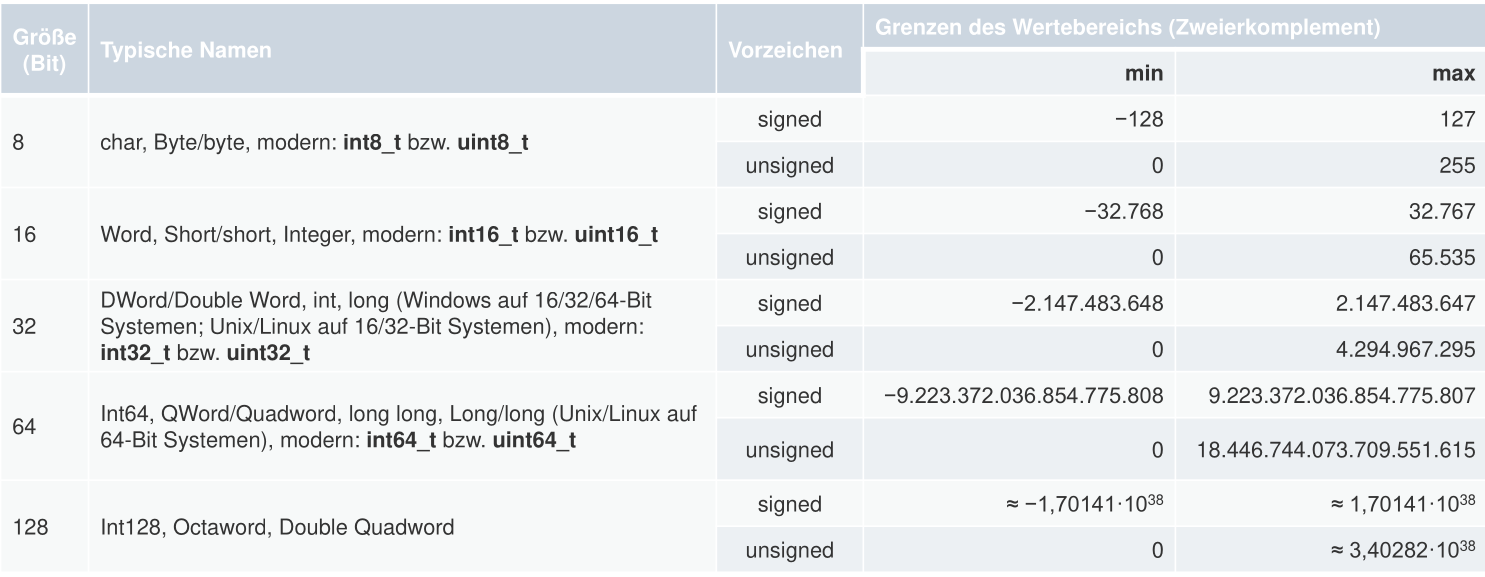
\includegraphics[scale=0.25]{pictures/types}
\end{figure}
\end{frame}

\section{Gleitkommazahlen}
\begin{frame}{Gleitkommazahlen}
Zur Darstellung von Zahlen, die betragsmäßig sehr groß oder sehr klein sind, verwendet man die Gleitkommadarstellung\\
Sie entspricht einer halblogarithmischen Form
$$
	X = \pm Mantisse \cdot q^{i}
$$
Die Basis $q$ ist für eine bestimmte Gleitkomma-Darstellung fest (meist 2 oder 16 Bit) und braucht damit nicht mehr explizit repräsentiert zu werden.\\
Gleitkommazahlen werden meist nicht im Zweierkomplement, sondern mit Betrag und Vorzeichen dargestellt.
\end{frame}

\subsection{Gleitkommazahlen}
\begin{frame}{Gleitkommazahlen}
\begin{itemize}
	\item Bei der Mantisse ist die Lage des Kommas wieder durch Vereinbarung festgelegt (meist links vom MSB)
	\item Der Exponent ist eine ganze Zahl, die in Form ihrer Charakteristik dargestellt wird
	\begin{itemize}
		\item Sowohl für die Charakteristik als auch für die Mantisse wird im Rechner eine feste Anzahl von Speicherstellen festgelegt
	\end{itemize}
	\item Die Länge der Charakteristik $y - x$ bestimmt die Größe des Zahlenbereichs
	\item Die Länge der Mantisse x bestimmt die Genauigkeit der Darstellung
\end{itemize}
\end{frame}

\begin{frame}{Gleitkomma-Maschinenformat}
\begin{figure}
	\center
	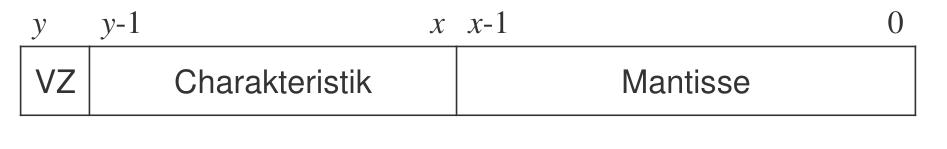
\includegraphics[scale=0.3]{pictures/g_maschine}
\end{figure}
$$
	\text{Dezimalzahl} = (-1)^{VZ} \cdot (0.\text{Mantisse}) \cdot q^{\text{Exponent}}
$$
$$
	\text{Exponent} = \text{Charakteristik} - q^{(y-1)-x}
$$
\end{frame}

\begin{frame}{Normalisierung}
\begin{itemize}
	\item Eine Gleitkommazahl heißt normalisiert, wenn für den Wert der Mantisse gilt:
	$$
		\frac{1}{q} \leq Mantisse < 1
	$$
	\item In dualer Darstellung ist die erste Stelle nach dem Komma gleich $1$, d.h. $(0,1 \ldots )$
	\item Ausnahme:\\
	Bei der Zahl 0 sind alle Stellen der Mantisse gleich Null
\end{itemize}
\end{frame}


\begin{frame}{Normalisierung}
\begin{itemize}
	\item Legt man für die Zahl $0$ ein spezielles Bitmuster fest, ist die erste Stelle der Mantisse in normalisierter Form immer gleich $1$
	\item Die erste Stelle der Mantisse braucht im Maschinenformat gar nicht erst dargestellt zu werden, d.h. $(0,1 \ldots)$
	\item \textcolor{red}{Man spart ein Bit bei der Speicherung oder gewinnt bei gleichem Speicherbedarf ein Bit an Genauigkeit}
	\item Bei arithmetischen Operationen und bei der Konversion in andere Darstellungen darf diese Stelle natürlich nicht vergessen werden
\end{itemize}
\end{frame}

\begin{frame}{Beispiel}
\begin{itemize}
	\item Darstellung der Zahl $7135_{10}$
	\item 3 verschiedene Maschinenformate mit je 32 Bit und $q = 2$
	\item Die Zahl $7135_{10}$ wird in jedem dieser Formate dargestellt.
	\begin{enumerate}
		\item Festkommadarstellung mit Zweierkomplement
		\begin{figure}
			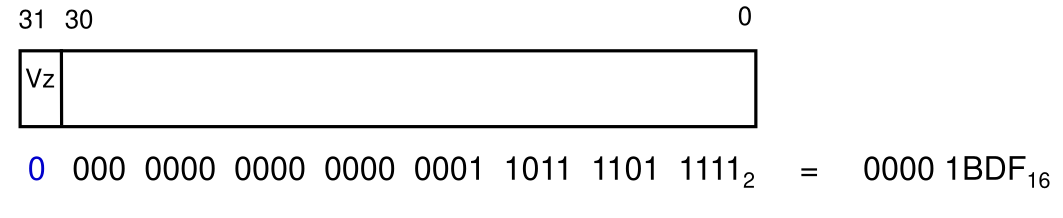
\includegraphics[scale=0.3]{pictures/festkomma}
		\end{figure}
	\end{enumerate}
\end{itemize}
\end{frame}

\begin{frame}{Beispiel}
	\begin{enumerate}\addtocounter{enumi}{1}
		\item Gleitkommadarstellung, normalisiert:
		\begin{figure}
			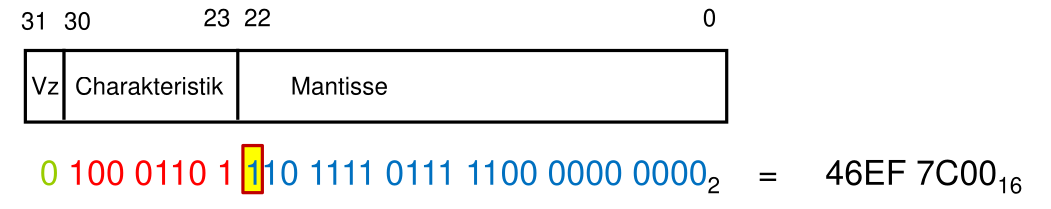
\includegraphics[scale=0.3]{pictures/norm}
		\end{figure}
		\item Gleitkommadarstellung, normalisiert, erste \enquote{1} implizit:
		\begin{figure}
			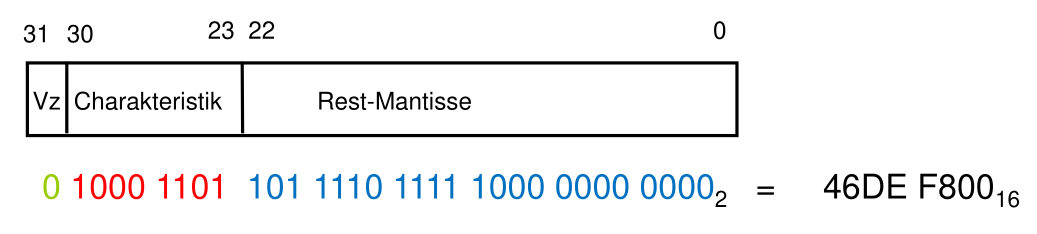
\includegraphics[scale=0.3]{pictures/norm_1}
		\end{figure}
	\end{enumerate}
\end{frame}

\subsection{Wertebereich}
\begin{frame}{Darstellbarer Zahlenbereich}
\begin{itemize}
	\item Die Anzahl darstellbarer Zahlen (Bitkombinationen) ist zwar in allen drei Fällen gleich $(2^{32})$
	\item \textcolor{red}{Der Bereich und damit die Dichte darstellbarer Zahlen auf dem Zahlenstrahl ist aber sehr unterschiedlich}
\end{itemize}
\end{frame}

\begin{frame}{Darstellbarer Zahlenbereich}
\begin{itemize}
	\item[1.)] Zahlen zwischen $-2^{31}$ und $2^{31}-1$
	\begin{figure}
		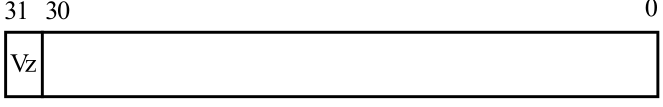
\includegraphics[scale=0.3]{pictures/format_a}
	\end{figure}
	\item[2.)]~\\
	\begin{itemize}
	\item negative Zahlen: $-(1-2^{-23}) \cdot 2^{127} \ldots -0.5 \cdot 2^{-128}$
	\item positive Zahlen: $0.5 \cdot 2^{-128} \ldots (1-2^{-23}) \cdot 2^{127}$
	\item Null
	\end{itemize}
	\begin{figure}
		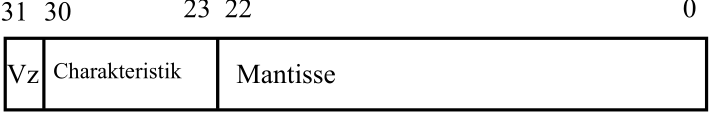
\includegraphics[scale=0.3]{pictures/format_b}
	\end{figure}
\end{itemize}
\end{frame}

\begin{frame}{Darstellbarer Zahlenbereich}
\begin{itemize}
	\item[3.)] normalisierte Gleitkommadarstellung
	\begin{itemize}
	\item negative Zahlen: $-(1-2^{-24}) \cdot 2^{127} \ldots -0.5 \cdot 2^{-128}$
	\item positive Zahlen: $0.5 \cdot 2^{-128} \ldots (1-2^{-24}) \cdot 2^{127}$
	\item \textcolor{red}{Die Null kann nicht dargestellt werden!}
	\end{itemize}
	\begin{figure}
		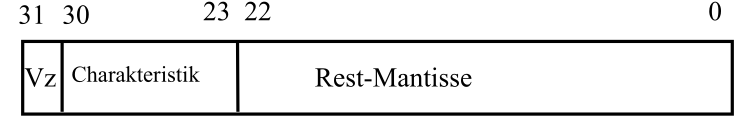
\includegraphics[scale=0.3]{pictures/format_c}
	\end{figure}
\end{itemize}
\end{frame}

\begin{frame}{Darstellbarer Zahlenbereich}
\begin{itemize}
	\item[1.)]~\\
	\begin{figure}
		\hspace*{0.21cm}
		
\includegraphics[scale=0.25]{pictures/f1}
	\end{figure}
	\item[2.)]~\\
	\vspace*{-1cm}
	\begin{figure}
		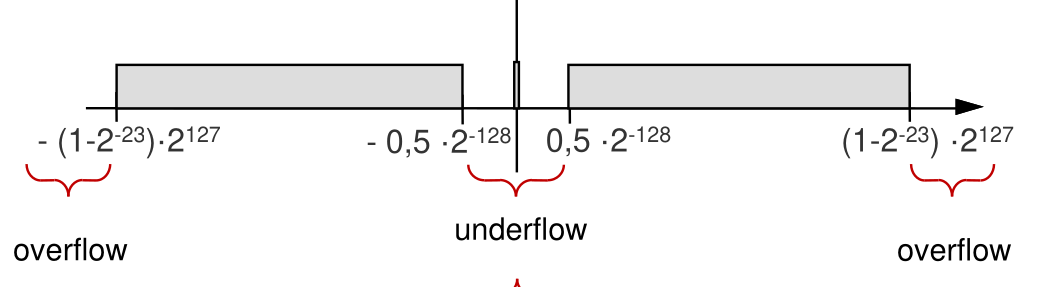
\includegraphics[scale=0.25]{pictures/f2}
	\end{figure}
	\item[3.)]~\\
	\vspace*{-1cm}
	\begin{figure}
		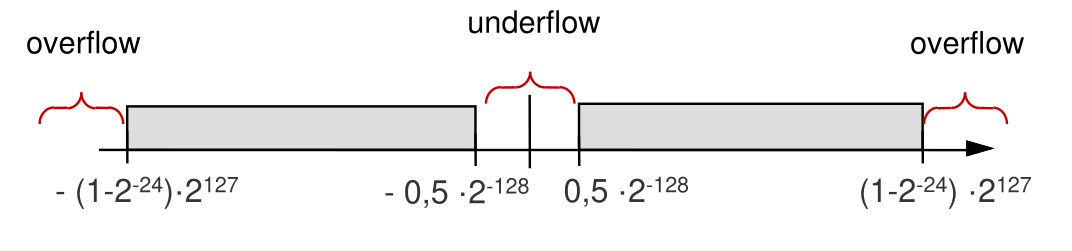
\includegraphics[scale=0.25]{pictures/f3}
	\end{figure}
\end{itemize}
\end{frame}

\subsection{Charakteristische Zahlen}
\begin{frame}{Charakteristische Zahlen}
\begin{itemize}
	\item Um verschiedene Gleitkommadarstellungen miteinander vergleichen zu können, definiert man drei
charakteristische Zahlen:
	\begin{itemize}
		\item \texttt{maxreal} ist die größte darstellbare normalisierte positive Zahl
		\item \texttt{minreal} ist die kleinste darstellbare normalisierte positive Zahl
		\item \texttt{smallreal} ist die kleinste Zahl, die man zu 1 addieren kann, um einen von 1 verschiedenen Wert zu erhalten
	\end{itemize}
\end{itemize}
\end{frame}

\begin{frame}{Charakteristische Zahlen -- Beispiel}
\begin{itemize}
	\item In Format 2.) im letzten Beispiel
	\begin{figure}
	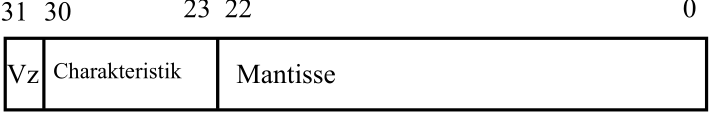
\includegraphics[scale=0.3]{pictures/format_b}
	\end{figure}
	\begin{itemize}
		\item maxreal = $(1 - 2-^{23})\cdot 2^{127}$
		\item minreal = $0.5 \cdot 2^{-128}$
	\end{itemize}
	\item Die Zahl $1$ wird normalisiert als $0.5 \cdot 2^1$ dargestellt
	\item Die nächstgrößere darstellbare Zahl hat in der Mantisse zusätzlich zur $1$ in Bit $22$ eine $1$ in Bit $0$
	\item smallreal $= 0.00000000000000000000001_2 \cdot 2^1$,
	\item also smallreal $= 2^{-23} \cdot 2^1 = 2^{-22}$
\end{itemize}
\end{frame}

\begin{frame}{Ungenauigkeiten}
\begin{itemize}
	\item Die Differenz zwischen zwei aufeinanderfolgenden Zahlen wächst bei Gleitkomma-Zahlen exponentiell mit der Größe der Zahlen, während sie bei Festkommazahlen konstant ist.
	\item Bei der Darstellung großer Zahlen ergibt sich damit auch eine hohe Ungenauigkeit
	\item Die Gesetzmäßigkeiten, die für reelle Zahlen gelten, werden für Maschinendarstellungen verletzt!
	\item (auch wenn diese Zahlen in einer höheren Programmiersprache oft \texttt{real} heißen).
\end{itemize}
\end{frame}

\begin{frame}{Ungenauigkeiten}
\begin{figure}
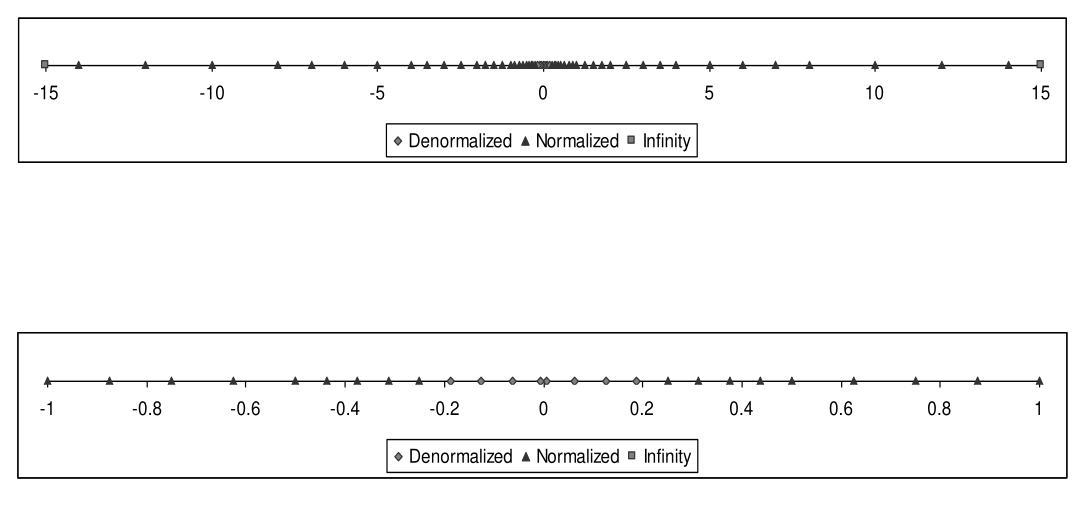
\includegraphics[scale=0.3]{pictures/ungenau}
\end{figure}
\end{frame}

\begin{frame}{Beispiel Ungenauigkeit}
\begin{itemize}
	\item Das Assoziativgesetz $(x + y) + z = x + (y + z)$ gilt selbst dann nicht allgemeingültig, wenn kein overflow oder underflow auftritt
	\begin{itemize}
		\item z.B.: $x = 1; y = z = smallreal/2$
		\begin{align*}
		(x + y) + z & = & (1 + smallreal/2) + smallreal/2 \\
		& = & 1 + smallreal/2 \\
		& = & 1 \\
		x + (y + z) & = & 1 + (smallreal/2 + smallreal/2)\\
		& = & 1 + smallreal\\
		& \neq & 1 
		\end{align*}
	\end{itemize}
\end{itemize}
\end{frame}


\section*{Quellen}
\appendix
\begin{frame}[allowframebreaks]
  \frametitle<presentation>{Quellen}
\printbibliography
\end{frame}
\end{document}